\appendix
\appendixpage
\addappheadtotoc





\chapter{Extension of scalars}





\section{Definition and universal property}


Let $L/k$ be a field extension. For a $k$-vector space $V$ we define
\[
 V_L := L \otimes_k V.
\]
Then $V_L$ is a $L$-vector space via
\[
 \lambda \cdot (l \otimes v) = (\lambda l) \otimes v
\]
for all $\lambda \in L$. To see that this multiplication is well-defined notice that for every $\lambda \in L$ the multiplication with $\lambda$ in $L$, namely
\[
 \pi_\lambda : L \to L, l \mapsto \lambda l,
\]
is $L$-linear and thus $k$-linear. The multiplication with $\lambda \in L$ as defined above is simply given by $\pi_\lambda \otimes \id_V$.

Given $k$-vector spaces $V$ and $W$ and a $k$-linear map $f : V \to W$. We get a $k$-linear map
\[
 f_L := \id_L \otimes f : V_L \to W_L.
\]
It is easy to check that $f_L$ is also $L$-linear. Therefore we can understand the extension of scalars as a functor from $\cVect{k}$ to $\cVect{L}$ which associates any $k$-vector space $V$ with $V_L$ and any $k$-linear map $f : V \to W$ with $f_L : V_L \to W_L$.

For any $k$-vector space $V$ we have a $k$-linear inclusion
\[
 \can_V : V \hookrightarrow V_L, v \mapsto 1 \otimes v.
\]


\begin{thrm}[Universal property of the extension of scalars]
 Let $V$ be a $k$-vector space. Then for every $L$-vector space $W$ we have a natural isomorphism of $k$-vector spaces
 \[
  \beta_W: \Hom_L(V_L, W) \to \Hom_k(V,W), f \mapsto f \circ \can_V.
 \]
 This property defines $V_L$ uniquely up to unique isomorphsm: If $V'$ is an $L$-vector space and $\iota : V \to V'$ a $k$-linear map such that
 \[
  \iota_W : \Hom_L(V', W) \to \Hom_k(V,W), f \mapsto f \circ \iota
 \]
 is an isomorphism of $k$-vector spaces for every $L$-vector space $W$ then there exists a unique isomorphism of $L$-vector spaces
 \[
  \phi : V_L \to V'
 \]
 such that the diagram
 \begin{center}
  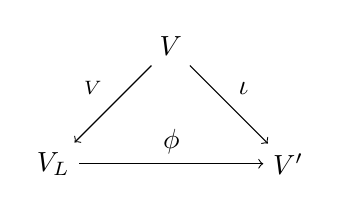
\begin{tikzpicture}[node distance = 6em, auto]
   \node (V) {$V$};
   \node (V_L) [below left of = V] {$V_L$};
   \node (V')  [below right of = V] {$V'$};
   \draw[->] (V) to node[swap] {$\can_V$} (V_L);
   \draw[->] (V) to node {$\iota$} (V');
   \draw[->] (V_L) to node {$\phi$} (V');
  \end{tikzpicture}
 \end{center}
 commutes.
\end{thrm}




